\documentclass[a4paper,11pt]{article}
\usepackage[%
  papersize={210mm,297mm},%
  layoutsize={200mm,270mm},%
  layoutoffset=5mm,%
  %twoside,%
  nomarginpar,%
  inner=25mm,%
  outer=25mm,%
  vmargin=25mm,%
  voffset=0mm,
  head=25mm,%
  headsep=25mm,%
  %includefoot,
  foot=25mm,%
  %includefoot,
  %showcrop,%
  %showframe,%
]{geometry}
\usepackage{titling}
\newcommand{\subtitle}[1]{%
  \posttitle{%
    \par\end{center}
    \begin{center}\large#1\end{center}
    \vskip0.5em}%
}
\usepackage[english]{babel}
\usepackage[T1]{fontenc}
\usepackage[utf8]{inputenc}
\usepackage{lmodern}
\usepackage[hidelinks]{hyperref}
\usepackage{graphicx}

\graphicspath{{./figures/}}

\begin{document}

\title{\vspace{-4em}\textbf{Comparison of constraints in different environments}}
\subtitle{\vspace{-2em}}
\author{Montiel Abello}
\date{\today}

\maketitle

\section{Overview}

Key results:
\begin{itemize}
\item planar constraints with long walls reduce drift;
\item segmented walls allow, and even increase drift;
\item when points lie loosely on planes and plane parameters are free to adjust themselves, angle constraints improve orthogonality.
\end{itemize}

Outstanding issues:
\begin{itemize}
\item when system gets large (>200 vertices, 1000 edges) and no loop closures occur (ie corridor, corner), gauss-newton takes many iterations to converge. 
\end{itemize}

\section{Results}
Simulation details:
\begin{itemize}
\item odometry, points measurement and plane angle constraint standard deviations were held constant
\item the same level of noise was used in generating measurements and in the estimation;
\item measurements were processed incrementally;
\item gauss-newton was used;
\item simulation was run with a) no constraints, b) planar constraints and c) planar and angle constraints;
\item simulation was run with two levels of $\sigma_{plane-plane-angle}$, ie points very close to planes \& points loosely on planes (ground truth).
\end{itemize}

%CORRIDOR
\begin{figure}
\centering
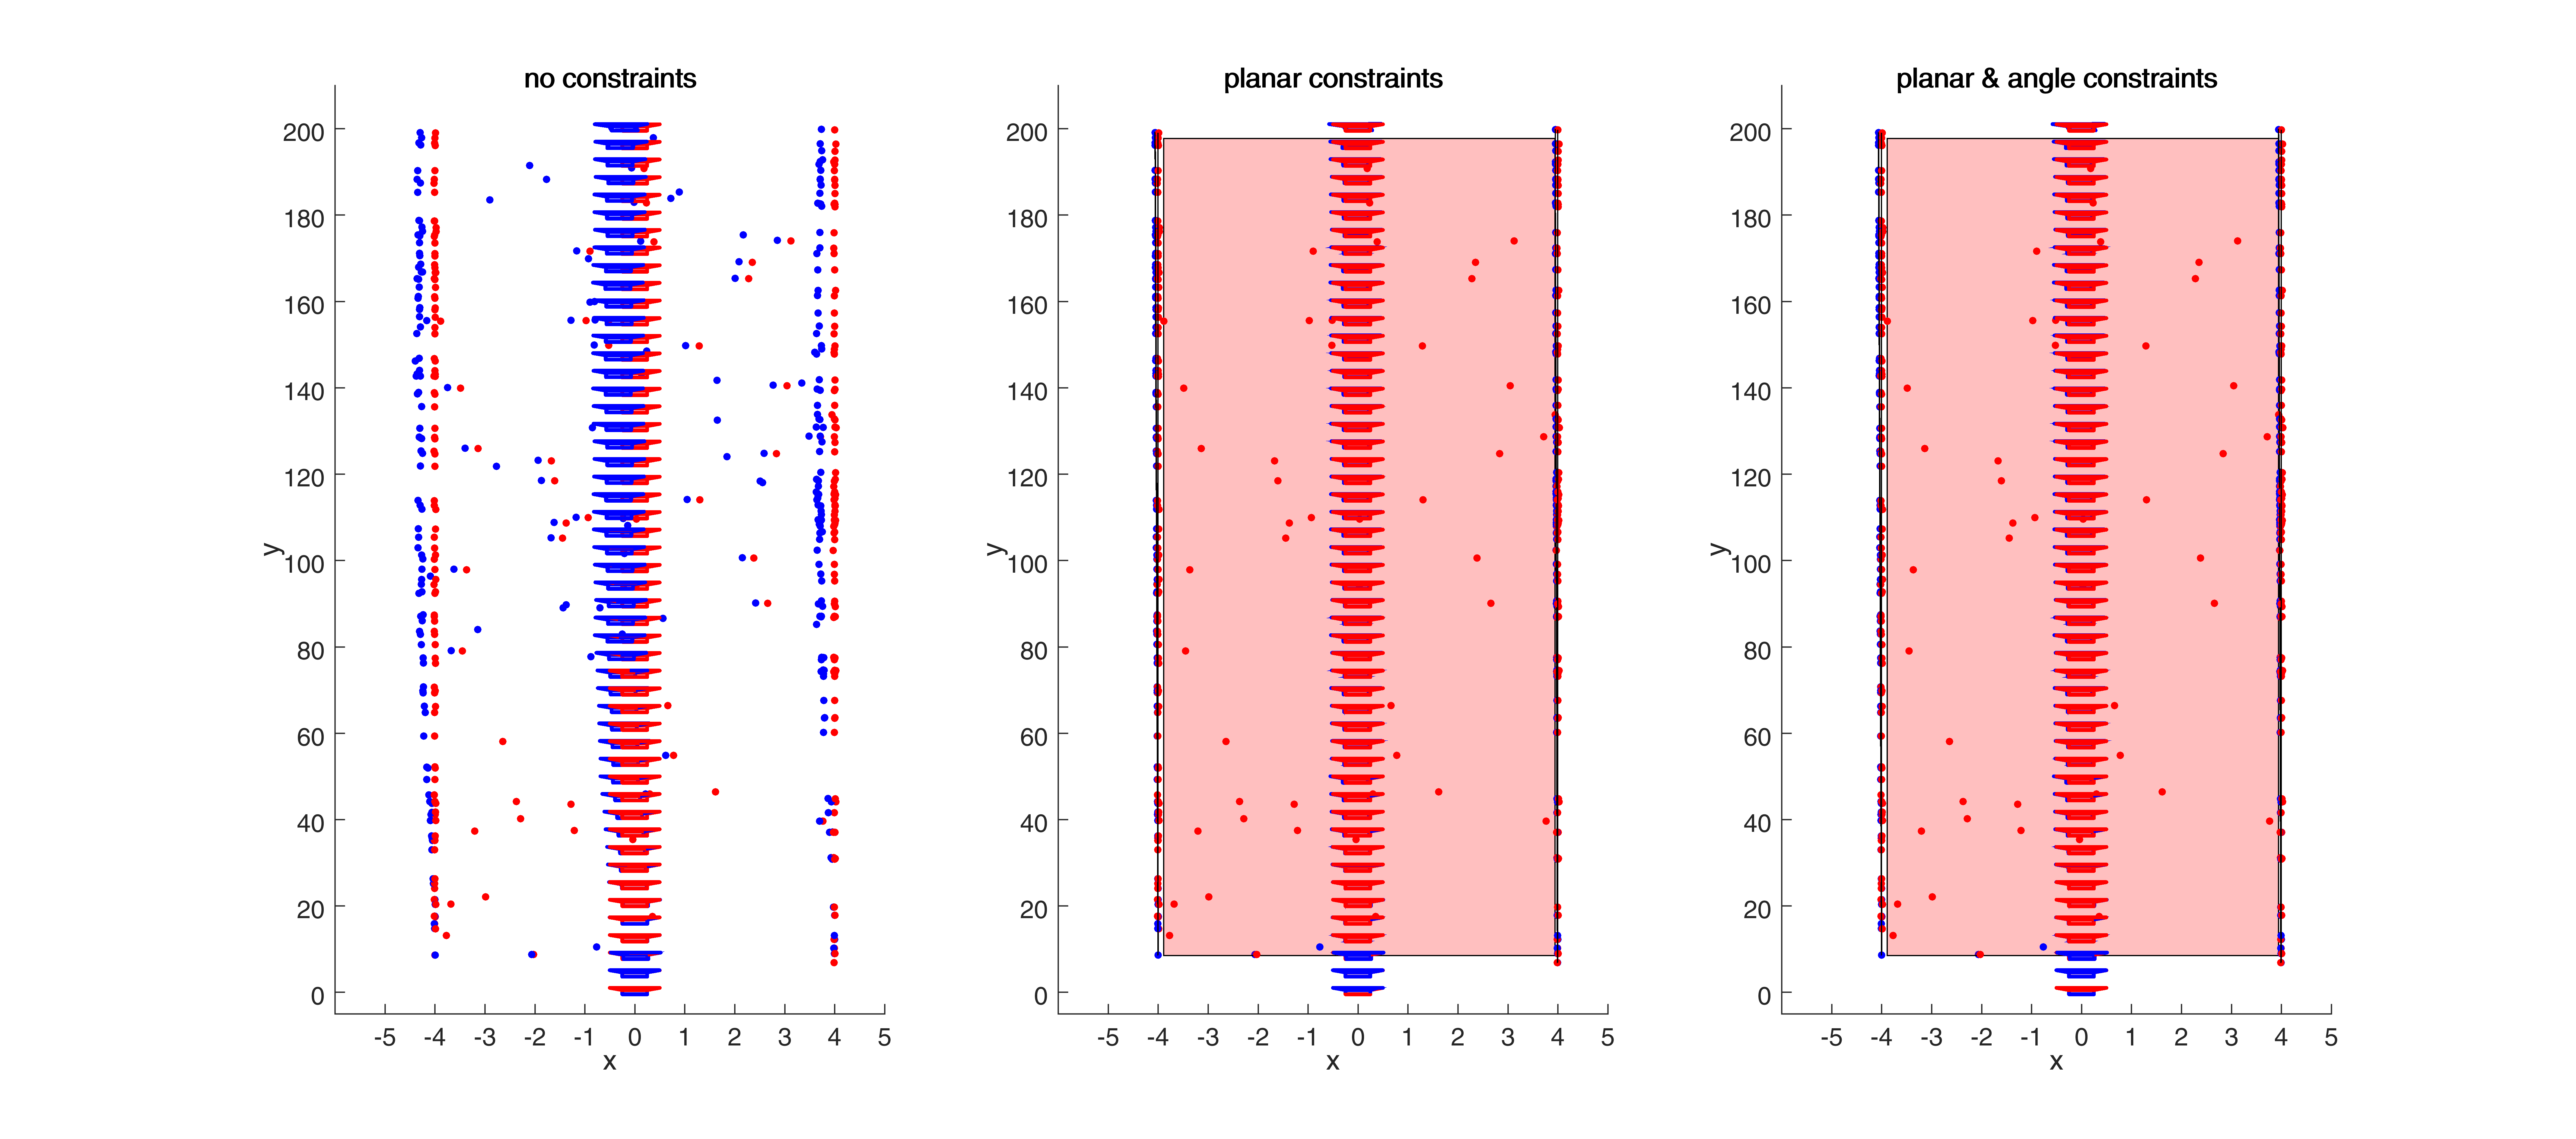
\includegraphics[width=1.15\textwidth,trim={3cm 0 0 0},clip]{corridorLowNoise.png}
\caption{\label{fig:corridorLowNoise} Comparison in corridor with ground, left and right planes (images not to scale). Points tightly distributed around planes. Angle constraints: left and right planes orthogonal to ground and parallel to one another. Drift is reduced by planar constraints.\newline
$\sigma_{odometry} = [0.02\textnormal{m},0.02\textnormal{m},0.02\textnormal{m},
\pi/90\textnormal{rad},\pi/90\textnormal{rad},\pi/90\textnormal{rad}]$\newline
$\sigma_{measurement} = [0.02\textnormal{m},0.02\textnormal{m},0.02\textnormal{m}]$\newline
$\sigma_{point-plane} = 0.01\textnormal{m}$\newline
$\sigma_{plane-plane-angle} = \pi/60\textnormal{rad}$}
\end{figure}

\begin{figure}
\centering
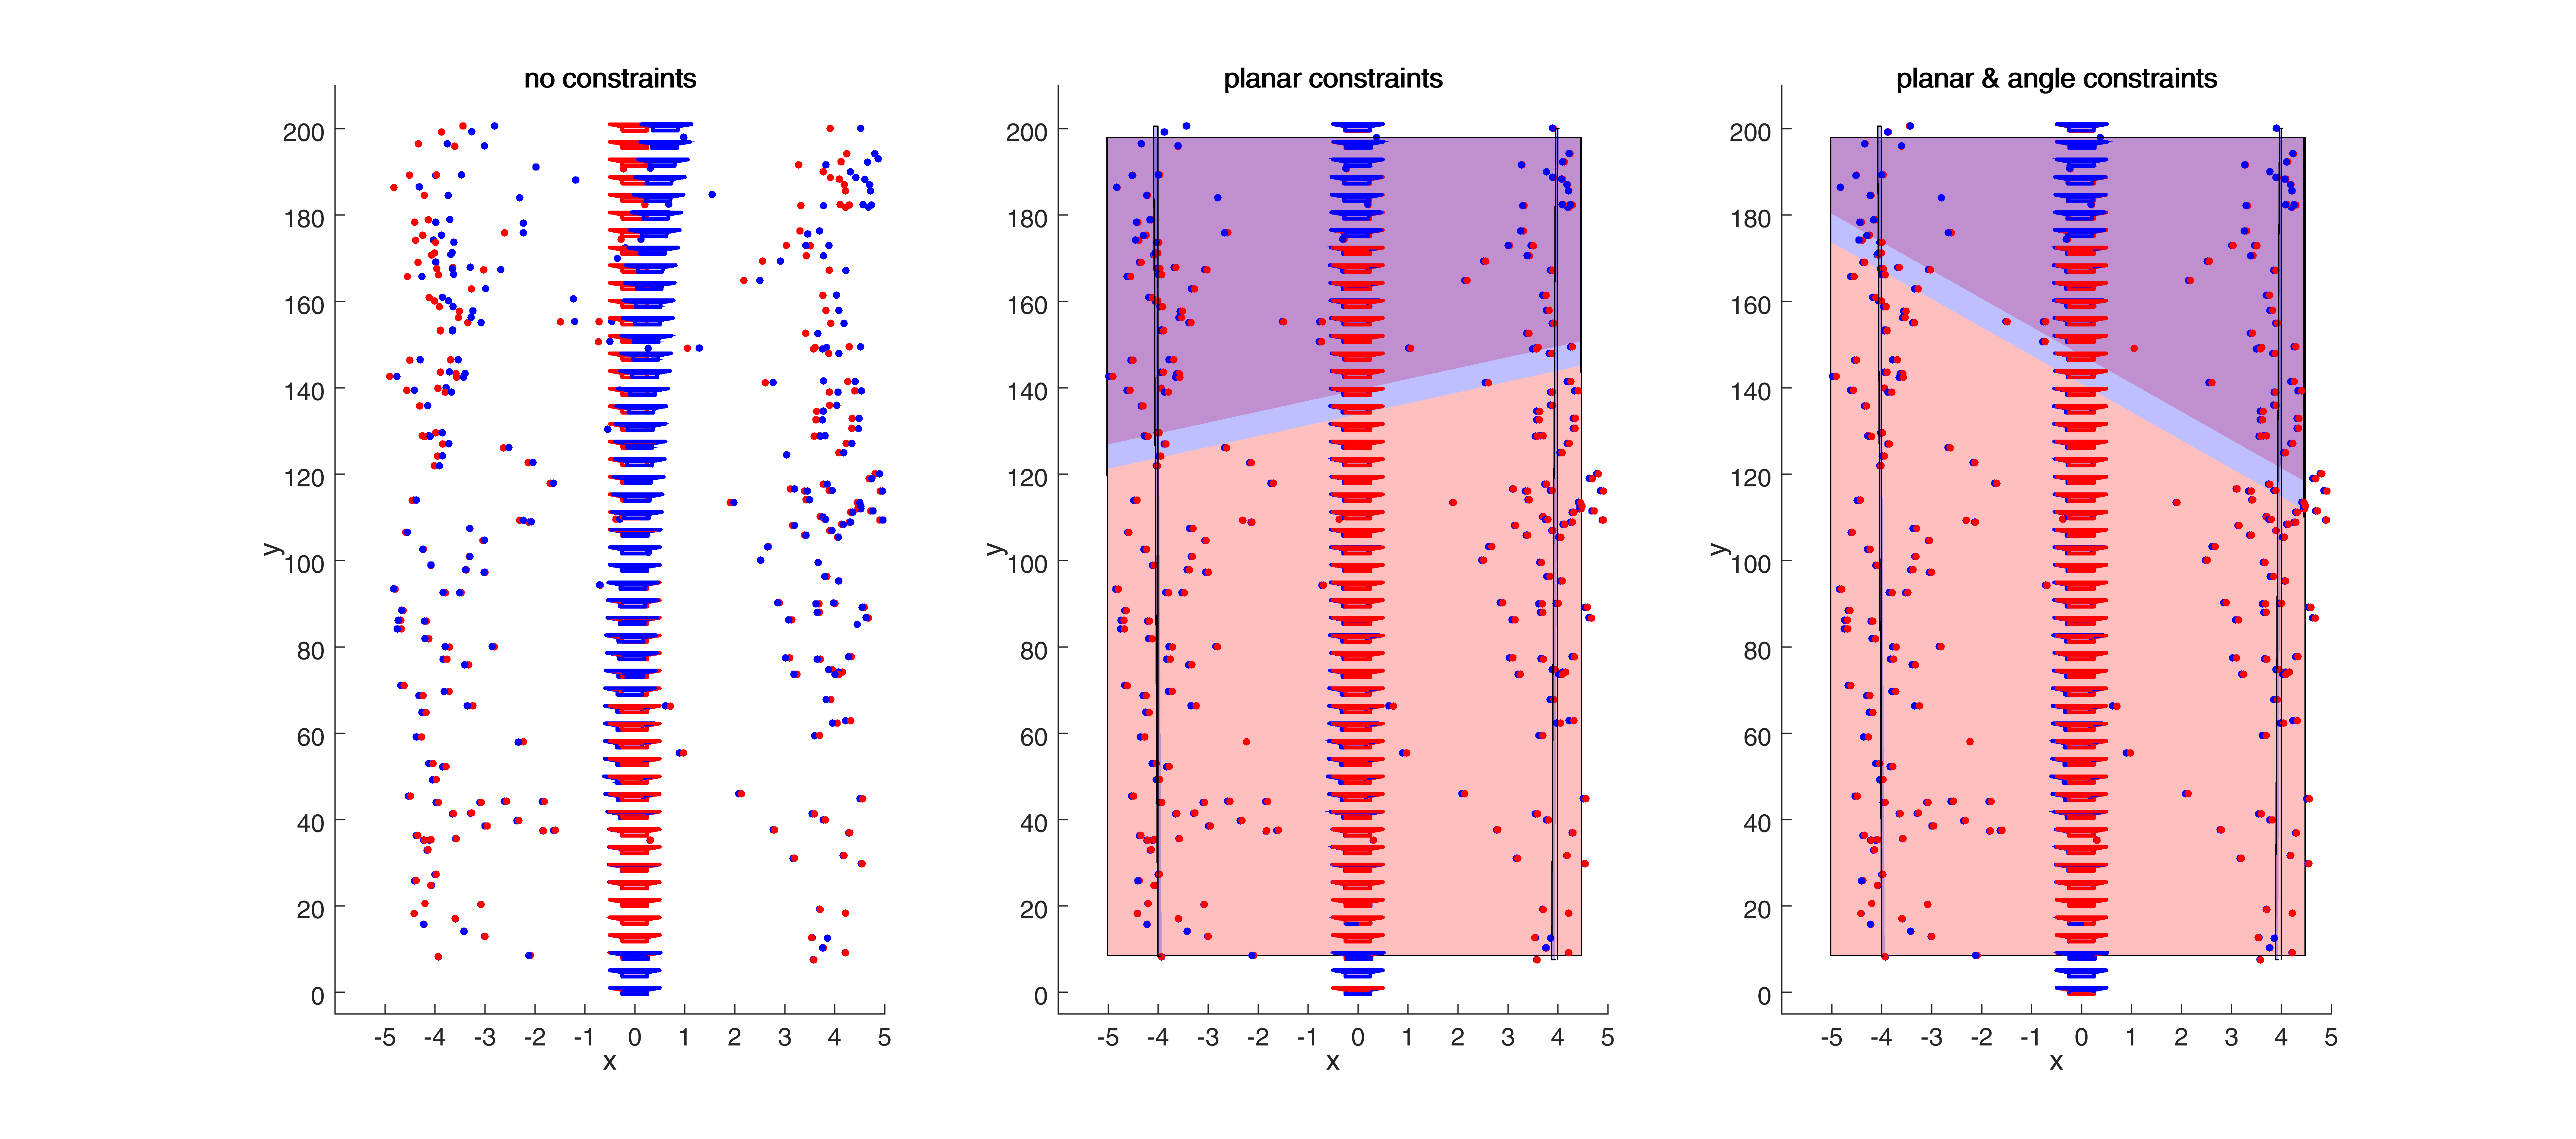
\includegraphics[width=1.15\textwidth,trim={3cm 0 0 0},clip]{corridorHighNoise.png}
\caption{\label{fig:corridorHighNoise} Comparison in corridor with ground, left and right planes (images not to scale). Points loosely distributed around planes. Angle constraints: left and right planes orthogonal to ground and parallel to one another. Drift is reduced by planar constraints.\newline
$\sigma_{odometry} = [0.02\textnormal{m},0.02\textnormal{m},0.02\textnormal{m},
\pi/90\textnormal{rad},\pi/90\textnormal{rad},\pi/90\textnormal{rad}]$\newline
$\sigma_{measurement} = [0.02\textnormal{m},0.02\textnormal{m},0.02\textnormal{m}]$\newline
$\sigma_{point-plane} = 0.5\textnormal{m}$\newline
$\sigma_{plane-plane-angle} = \pi/60\textnormal{rad}$}
\end{figure}

%SEGMENTED CORRIDOR
\begin{figure}
\centering
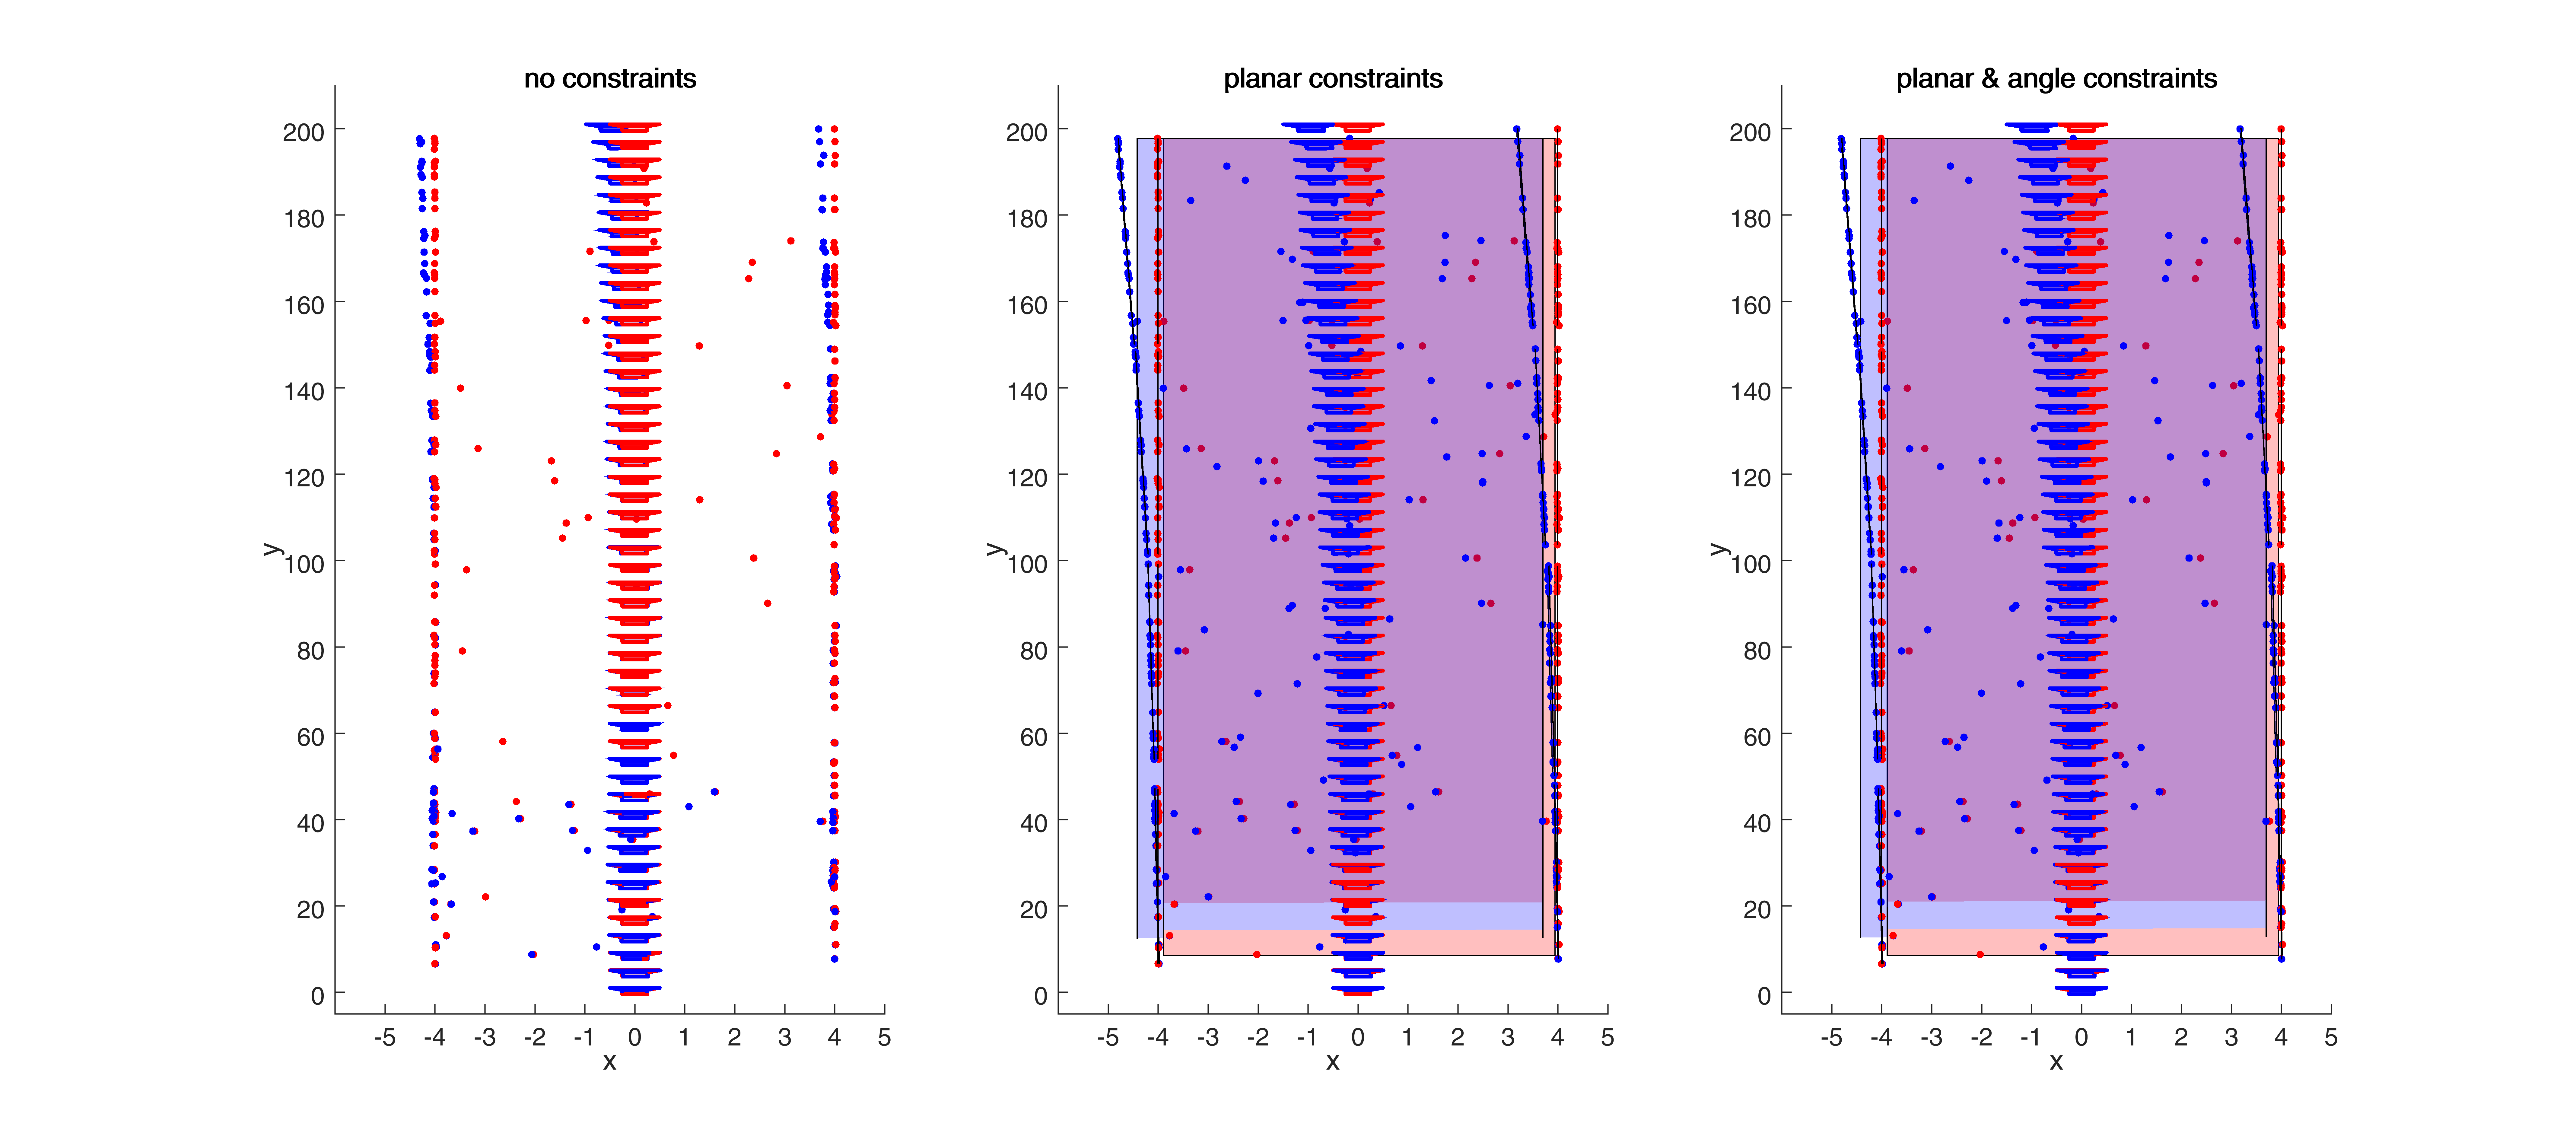
\includegraphics[width=1.15\textwidth,trim={3cm 0 0 0},clip]{segmentedCorridorLowNoise.png}
\caption{\label{fig:segmentedCorridorLowNoise} Comparison in corridor with ground, 4 left and 4 right planes (images not to scale). Points tightly distributed around planes. Angle constraints: wall planes orthogonal to ground and parallel to directly opposite plane. Drift is not reduce by planar constraints - seems to be increasing based on figure but this is due to random seed differing, due to different system sizes. More trials show drift is the same..\newline
$\sigma_{odometry} = [0.02\textnormal{m},0.02\textnormal{m},0.02\textnormal{m},
\pi/90\textnormal{rad},\pi/90\textnormal{rad},\pi/90\textnormal{rad}]$\newline
$\sigma_{measurement} = [0.02\textnormal{m},0.02\textnormal{m},0.02\textnormal{m}]$\newline
$\sigma_{point-plane} = 0.01\textnormal{m}$\newline
$\sigma_{plane-plane-angle} = \pi/60\textnormal{rad}$}
\end{figure}

\begin{figure}
\centering
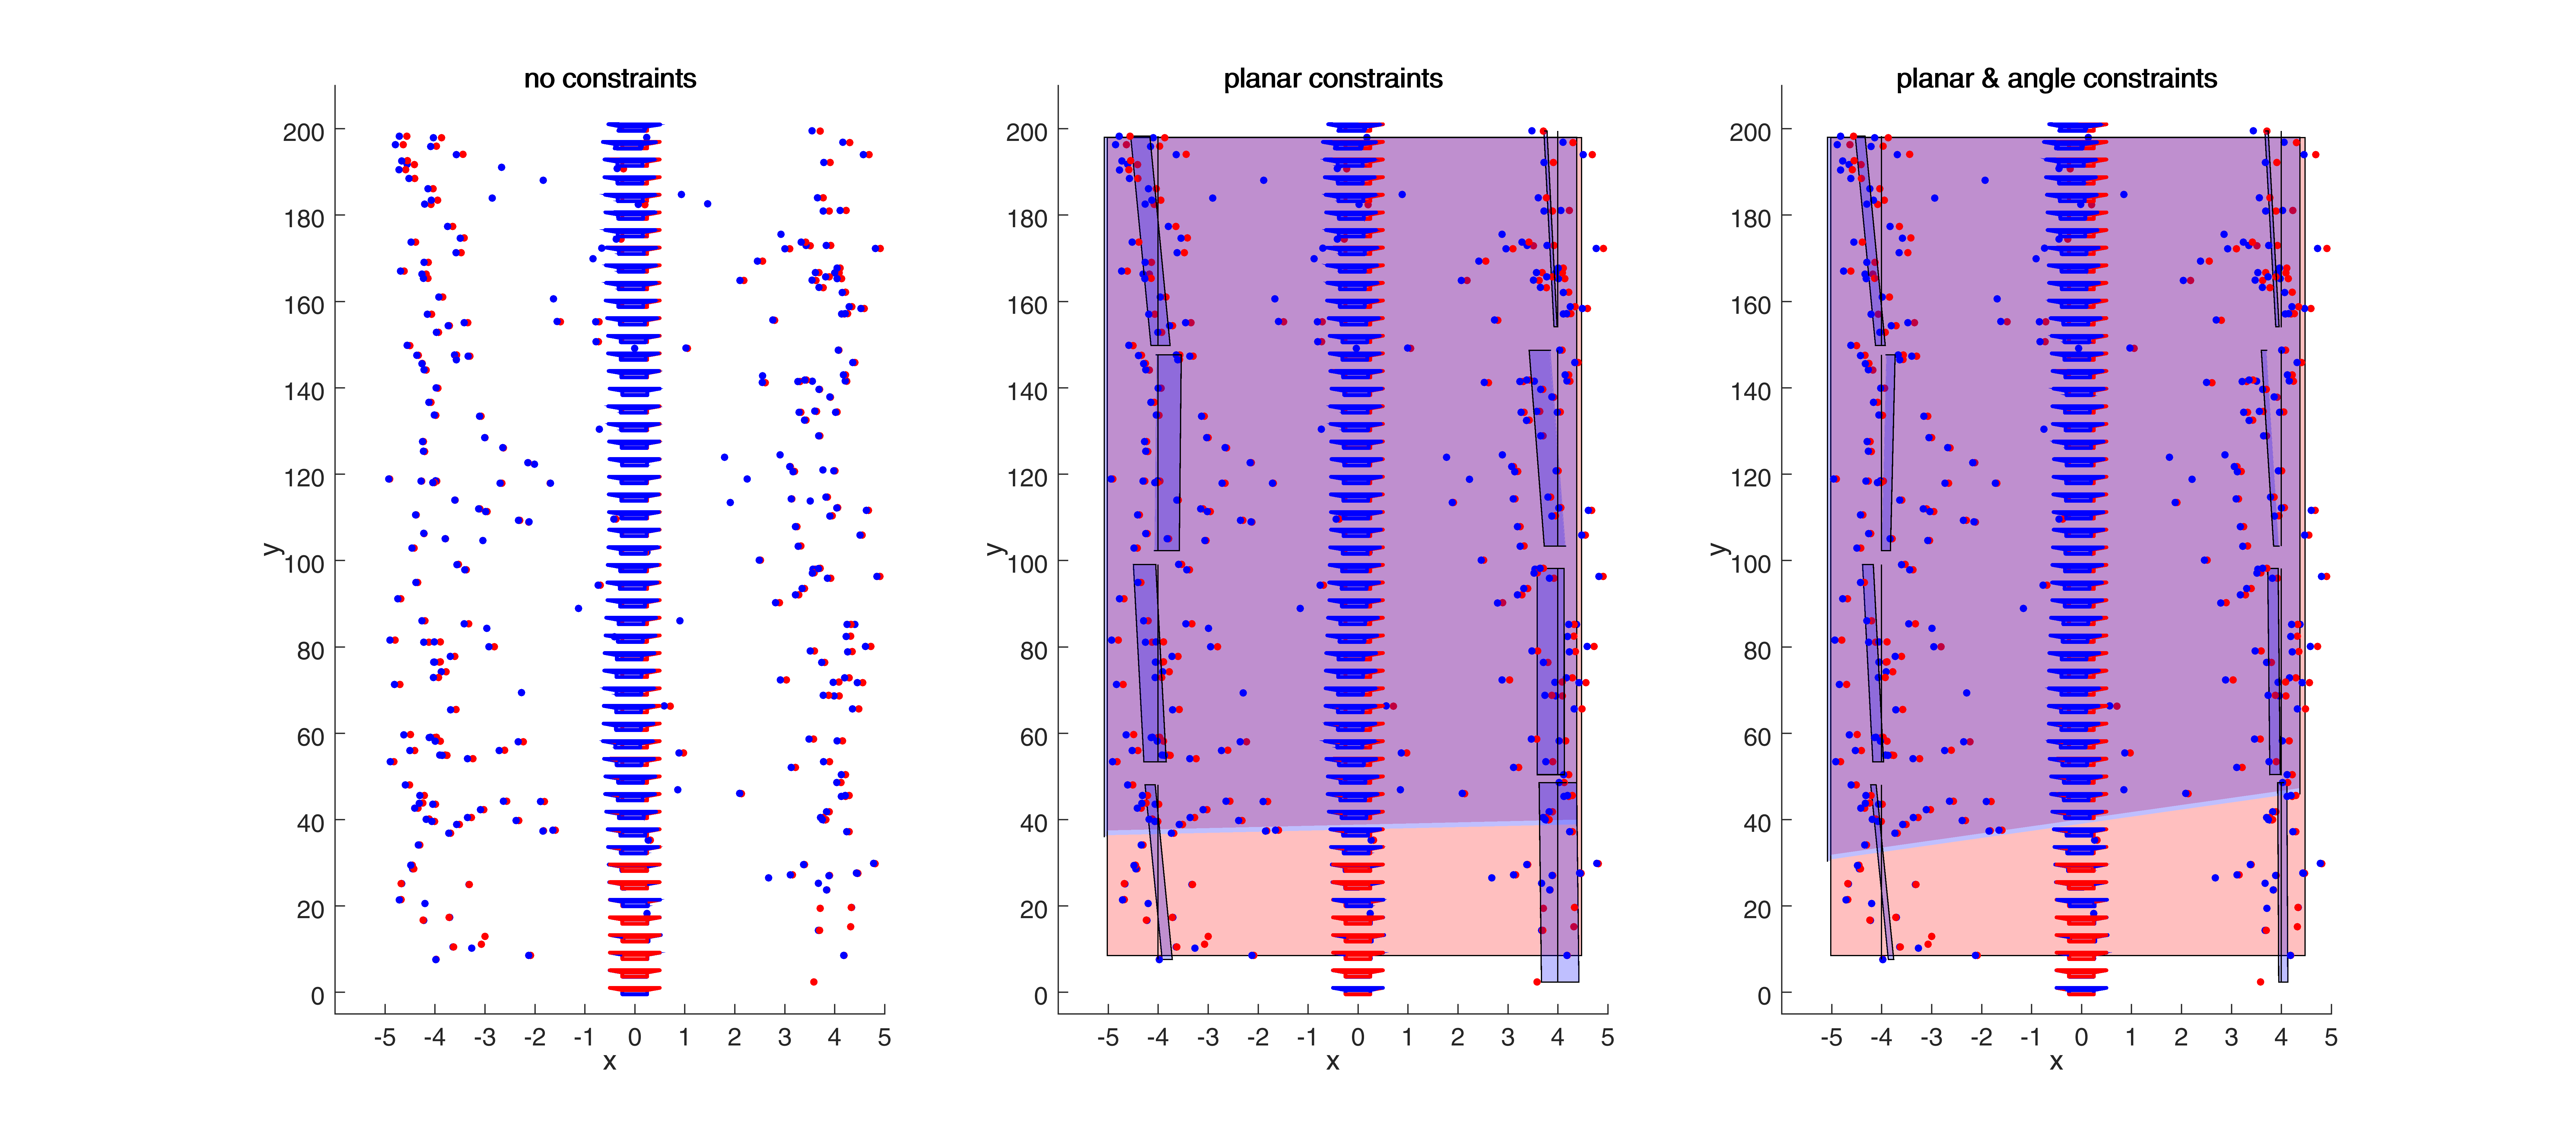
\includegraphics[width=1.15\textwidth,trim={3cm 0 0 0},clip]{segmentedCorridorHighNoise.png}
\caption{\label{fig:segmentedCorridorHighNoise} Comparison in corridor with ground, 4 left and 4 right planes (images not to scale). Points loosely distributed around planes. Angle constraints: wall planes orthogonal to ground and parallel to directly opposite plane. Angle constraints improve orthogonality of walls with ground.\newline
$\sigma_{odometry} = [0.02\textnormal{m},0.02\textnormal{m},0.02\textnormal{m},
\pi/90\textnormal{rad},\pi/90\textnormal{rad},\pi/90\textnormal{rad}]$\newline
$\sigma_{measurement} = [0.02\textnormal{m},0.02\textnormal{m},0.02\textnormal{m}]$\newline
$\sigma_{point-plane} = 0.5\textnormal{m}$\newline
$\sigma_{plane-plane-angle} = \pi/60\textnormal{rad}$}
\end{figure}

%CONNECTED SEGMENTED CORRIDOR
\begin{figure}
\centering
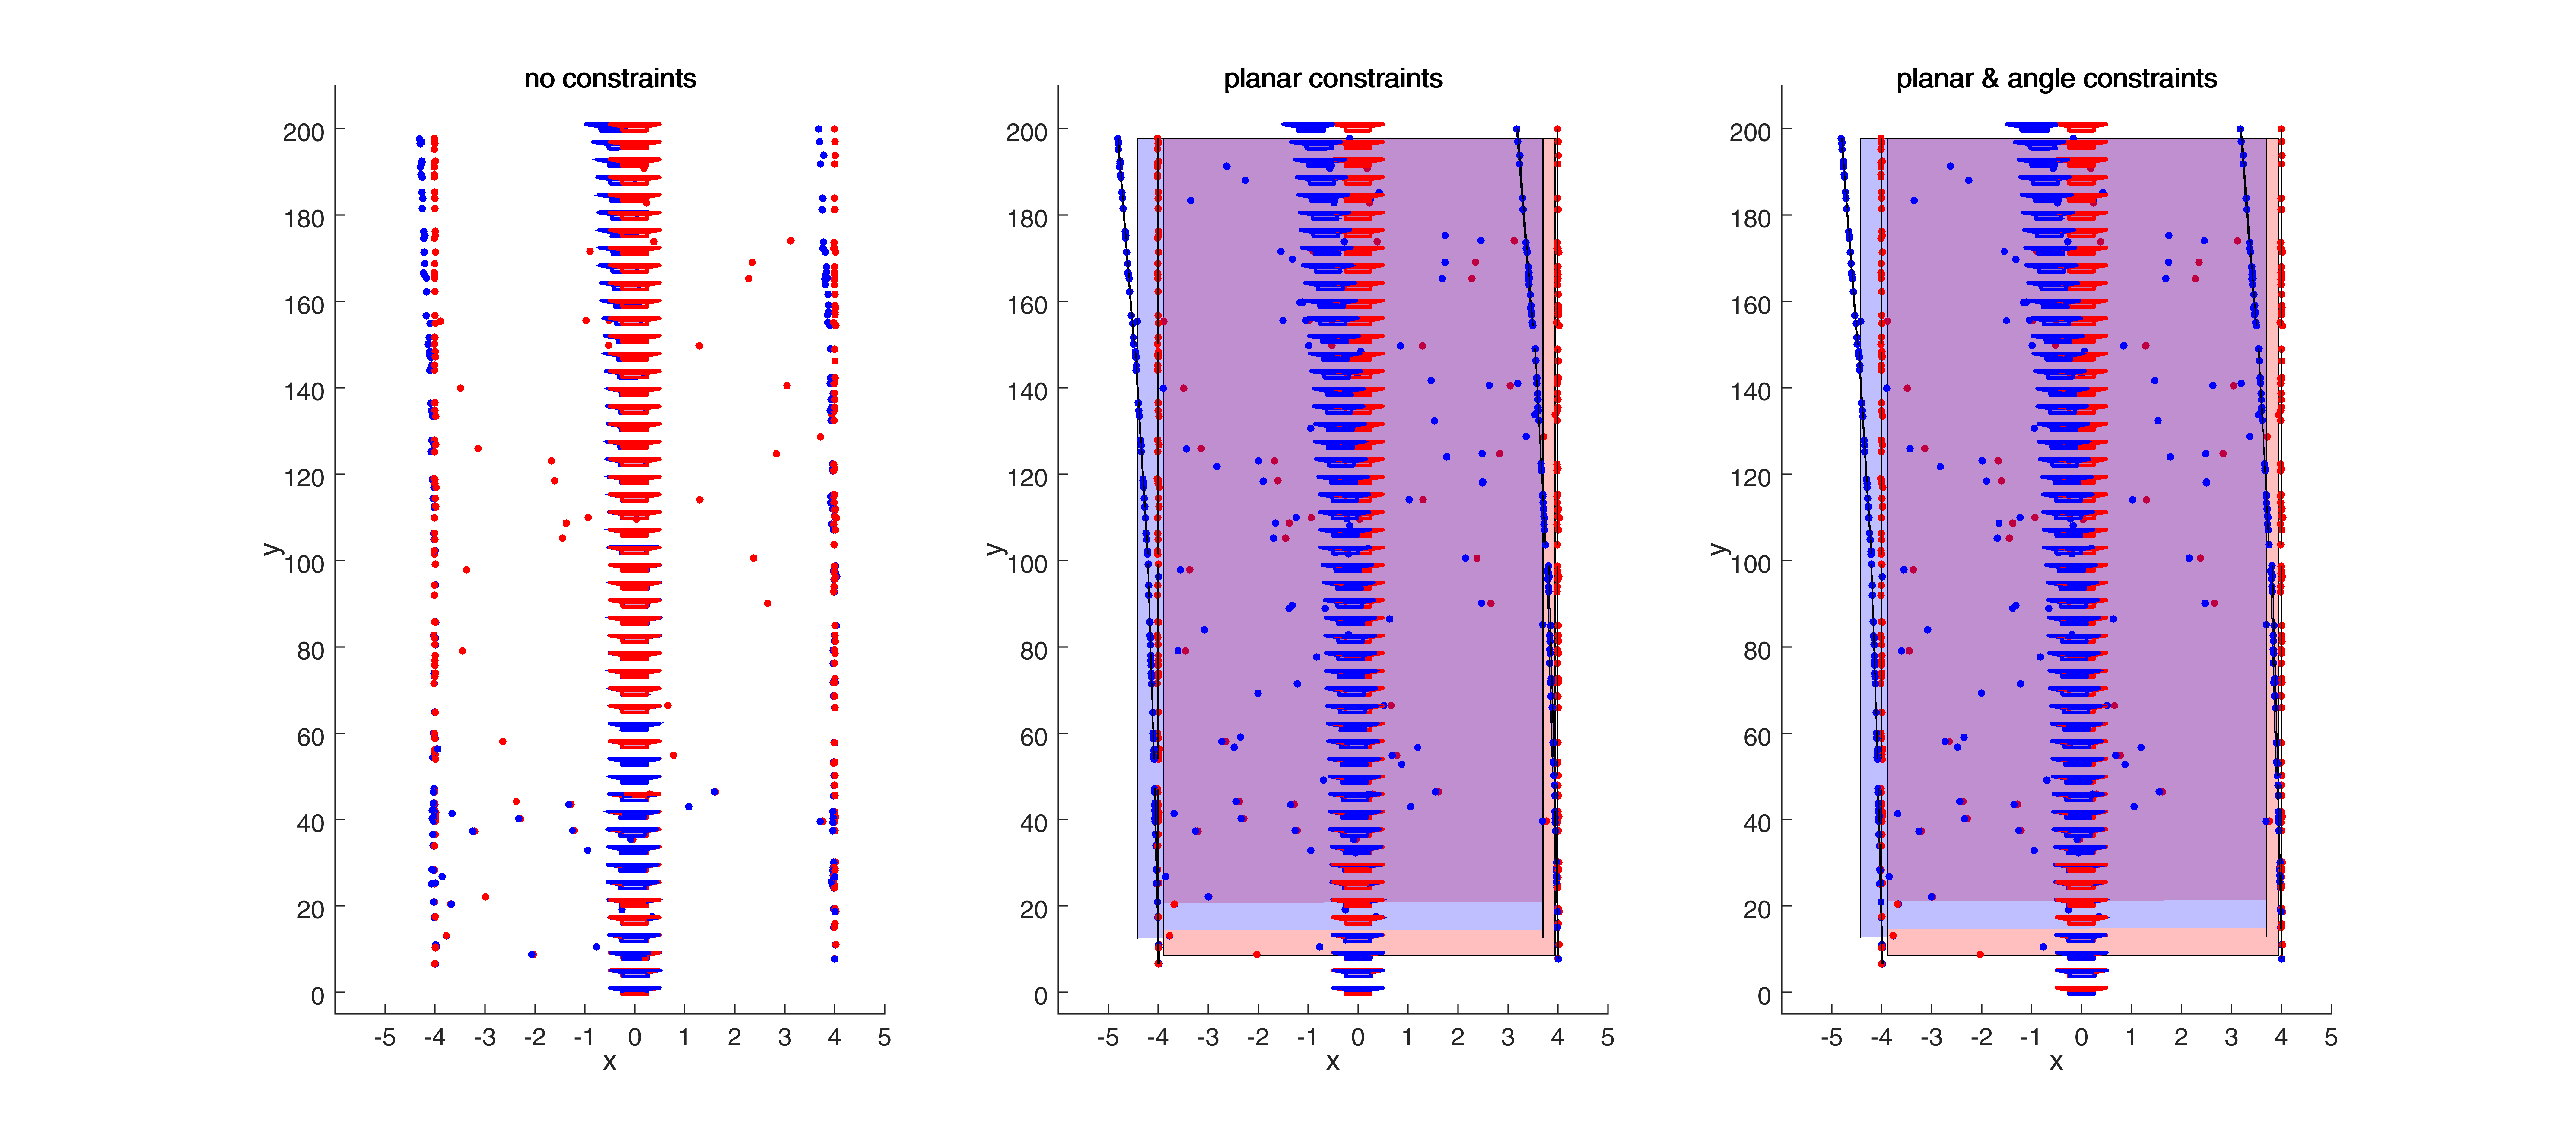
\includegraphics[width=1.15\textwidth,trim={3cm 0 0 0},clip]{connectedSegmentedCorridorLowNoise.png}
\caption{\label{fig:connectedSegmentedCorridorLowNoise} Comparison in corridor with ground, 4 left and 4 right planes (images not to scale). Points tightly distributed around planes. Angle constraints: wall planes orthogonal to ground and parallel to 3 closest opposite planes. Adding more angle constraints has no effect. Further tests showed that reducing $\sigma_{plane-plane-angle}$ had no effect either.\newline
$\sigma_{odometry} = [0.02\textnormal{m},0.02\textnormal{m},0.02\textnormal{m},
\pi/90\textnormal{rad},\pi/90\textnormal{rad},\pi/90\textnormal{rad}]$\newline
$\sigma_{measurement} = [0.02\textnormal{m},0.02\textnormal{m},0.02\textnormal{m}]$\newline
$\sigma_{point-plane} = 0.01\textnormal{m}$\newline
$\sigma_{plane-plane-angle} = \pi/60\textnormal{rad}$}
\end{figure}

\begin{figure}
\centering
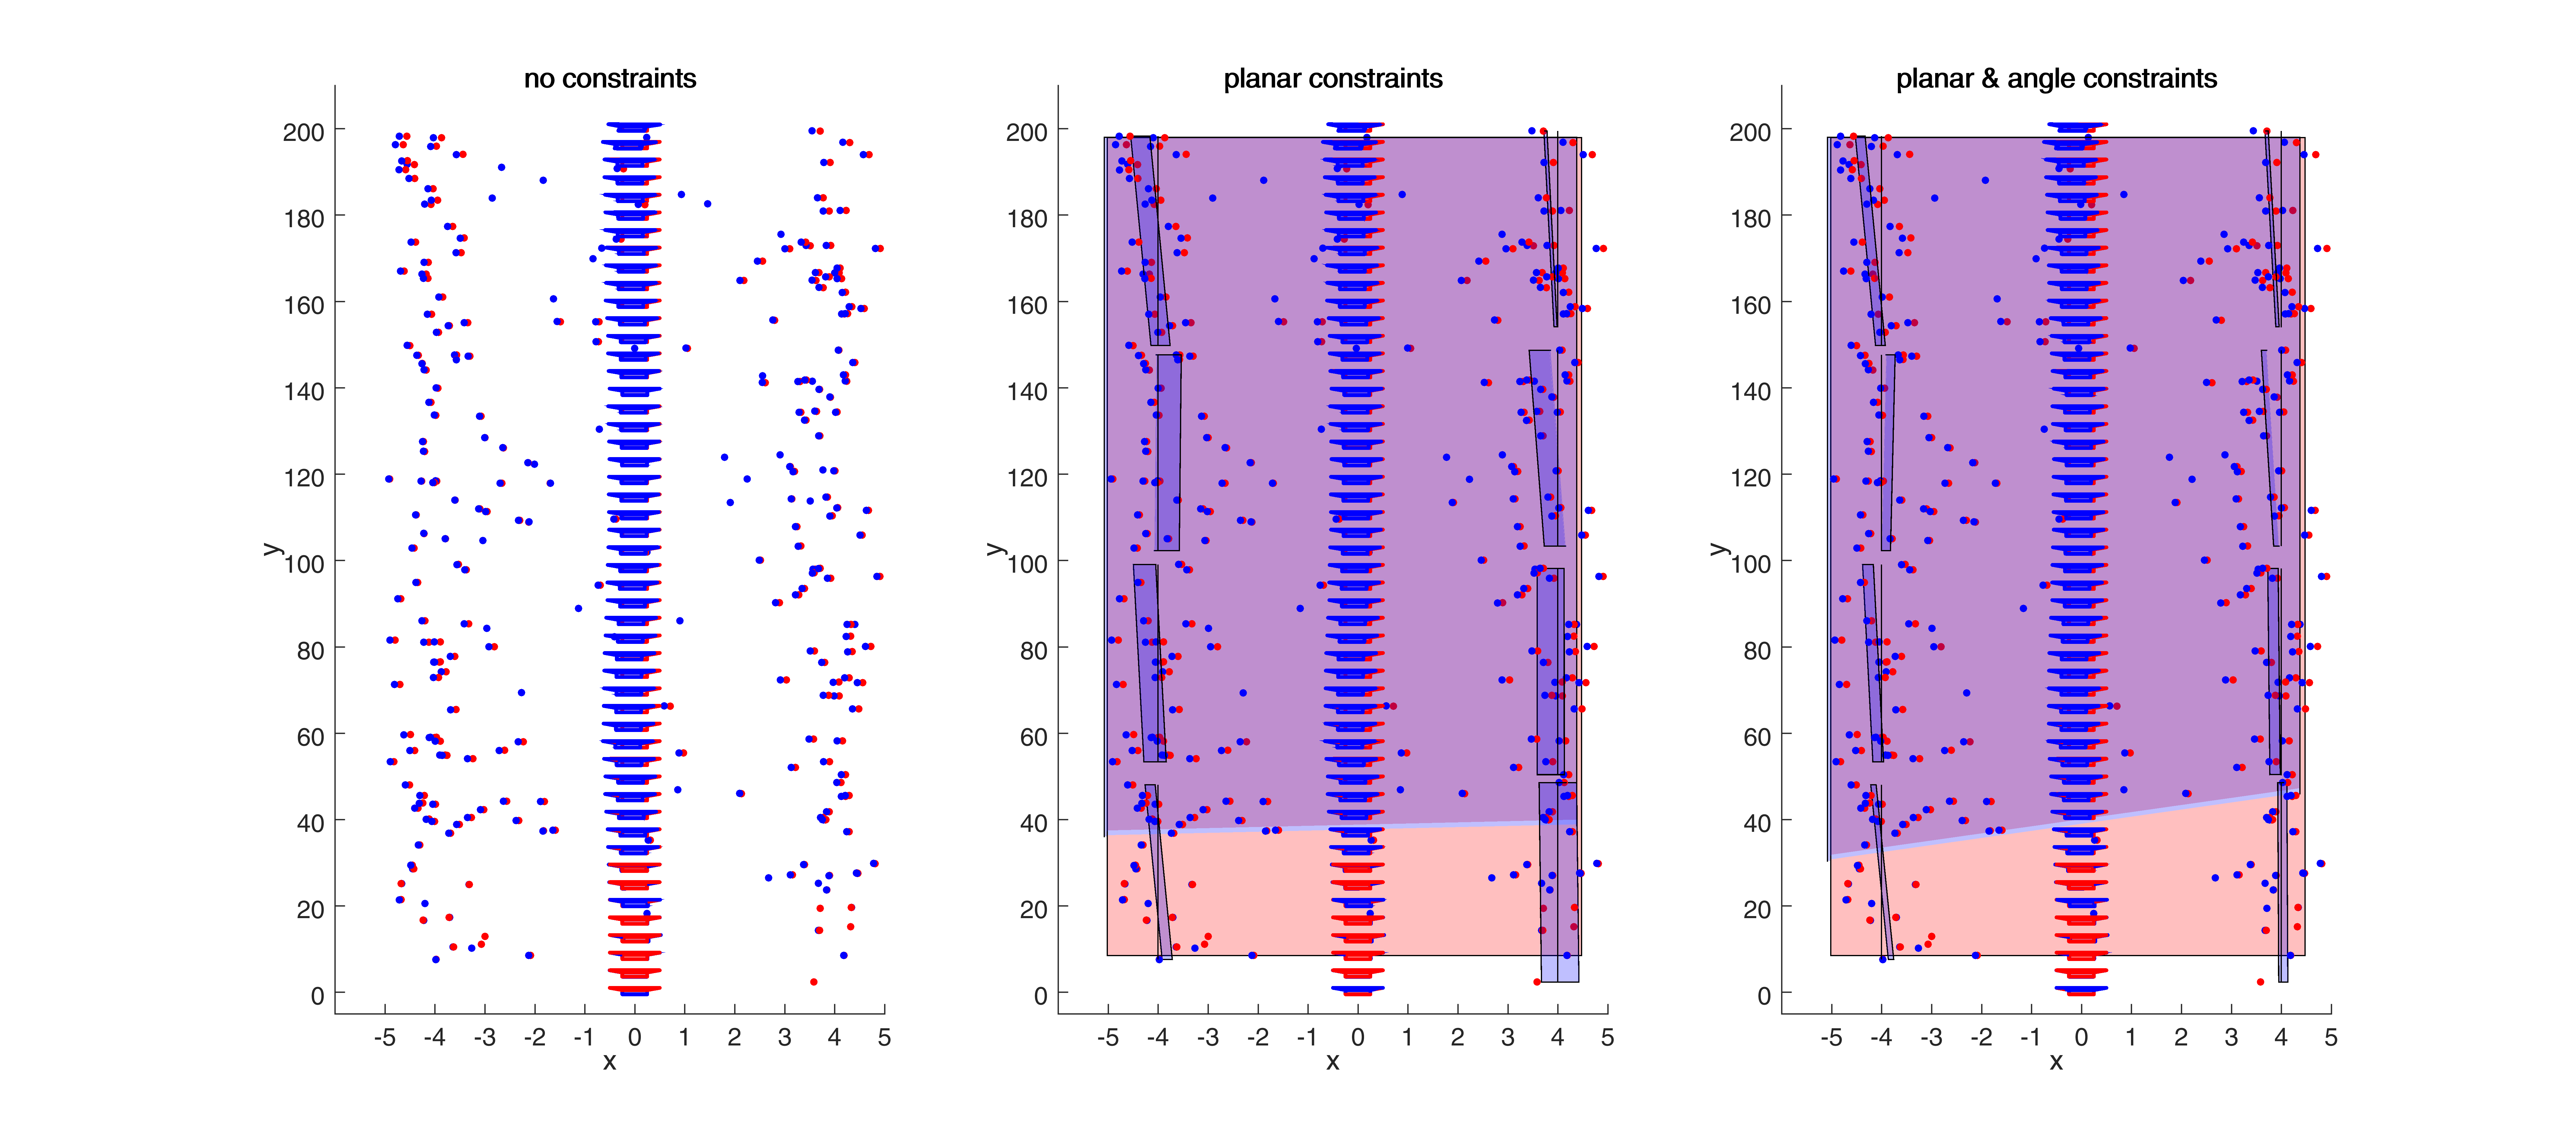
\includegraphics[width=1.15\textwidth,trim={3cm 0 0 0},clip]{connectedSegmentedCorridorHighNoise.png}
\caption{\label{fig:connectedSegmentedCorridorHighNoise} Comparison in corridor with ground, 4 left and 4 right planes (images not to scale). Points loosely distributed around planes. Angle constraints: wall planes orthogonal to ground and parallel to 3 closest opposite planes. Drift lower with no constraints. Adding more angle constraints has no effect. Further tests showed that reducing $\sigma_{plane-plane-angle}$ had no effect either. \newline
$\sigma_{odometry} = [0.02\textnormal{m},0.02\textnormal{m},0.02\textnormal{m},
\pi/90\textnormal{rad},\pi/90\textnormal{rad},\pi/90\textnormal{rad}]$\newline
$\sigma_{measurement} = [0.02\textnormal{m},0.02\textnormal{m},0.02\textnormal{m}]$\newline
$\sigma_{point-plane} = 0.5\textnormal{m}$\newline
$\sigma_{plane-plane-angle} = \pi/60\textnormal{rad}$}
\end{figure}

%CORNER
\begin{figure}
\centering
\includegraphics[width=1.15\textwidth,trim={3cm 0 0 0},clip]{cornerLowNoise.png}
\caption{\label{fig:cornerLowNoise} Comparison in corner with ground, 2 left and 2 right planes (images not to scale). Points tightly distributed around planes. Angle constraints: wall planes orthogonal to ground and parallel to opposite plane and orthogonal to connected plane. Planar constraints reduce drift. \newline
$\sigma_{odometry} = [0.02\textnormal{m},0.02\textnormal{m},0.02\textnormal{m},
\pi/90\textnormal{rad},\pi/90\textnormal{rad},\pi/90\textnormal{rad}]$\newline
$\sigma_{measurement} = [0.02\textnormal{m},0.02\textnormal{m},0.02\textnormal{m}]$\newline
$\sigma_{point-plane} = 0.01\textnormal{m}$\newline
$\sigma_{plane-plane-angle} = \pi/60\textnormal{rad}$}
\end{figure}

\begin{figure}
\centering
\includegraphics[width=1.15\textwidth,trim={3.5cm 0 0 0},clip]{cornerHighNoise.png}
\caption{\label{fig:cornerHighNoise} Comparison in corridor with ground, 4 left and 4 right planes (images not to scale). Points loosely distributed around planes. Angle constraints: wall planes orthogonal to ground and parallel to opposite plane and orthogonal to connected plane. \newline
$\sigma_{odometry} = [0.02\textnormal{m},0.02\textnormal{m},0.02\textnormal{m},
\pi/90\textnormal{rad},\pi/90\textnormal{rad},\pi/90\textnormal{rad}]$\newline
$\sigma_{measurement} = [0.02\textnormal{m},0.02\textnormal{m},0.02\textnormal{m}]$\newline
$\sigma_{point-plane} = 0.5\textnormal{m}$\newline
$\sigma_{plane-plane-angle} = \pi/60\textnormal{rad}$}
\end{figure}

\end{document}
              
            